\documentclass[11pt,ignorenonframetext,]{beamer}
\setbeamertemplate{caption}[numbered]
\setbeamertemplate{caption label separator}{: }
\setbeamercolor{caption name}{fg=normal text.fg}
\beamertemplatenavigationsymbolsempty
\usepackage{lmodern}
\usepackage{amssymb,amsmath}
\usepackage{ifxetex,ifluatex}
\usepackage{fixltx2e} % provides \textsubscript
\ifnum 0\ifxetex 1\fi\ifluatex 1\fi=0 % if pdftex
  \usepackage[T1]{fontenc}
  \usepackage[utf8]{inputenc}
\else % if luatex or xelatex
  \ifxetex
    \usepackage{mathspec}
  \else
    \usepackage{fontspec}
  \fi
  \defaultfontfeatures{Ligatures=TeX,Scale=MatchLowercase}
\fi
\usetheme[]{metropolis}
% use upquote if available, for straight quotes in verbatim environments
\IfFileExists{upquote.sty}{\usepackage{upquote}}{}
% use microtype if available
\IfFileExists{microtype.sty}{%
\usepackage{microtype}
\UseMicrotypeSet[protrusion]{basicmath} % disable protrusion for tt fonts
}{}
\newif\ifbibliography
\hypersetup{
            pdftitle={Lecture 9},
            pdfauthor={Colin Rundel},
            pdfborder={0 0 0},
            breaklinks=true}
\urlstyle{same}  % don't use monospace font for urls
\usepackage{color}
\usepackage{fancyvrb}
\newcommand{\VerbBar}{|}
\newcommand{\VERB}{\Verb[commandchars=\\\{\}]}
\DefineVerbatimEnvironment{Highlighting}{Verbatim}{commandchars=\\\{\}}
% Add ',fontsize=\small' for more characters per line
\newenvironment{Shaded}{}{}
\newcommand{\KeywordTok}[1]{\textcolor[rgb]{0.00,0.44,0.13}{\textbf{#1}}}
\newcommand{\DataTypeTok}[1]{\textcolor[rgb]{0.56,0.13,0.00}{#1}}
\newcommand{\DecValTok}[1]{\textcolor[rgb]{0.25,0.63,0.44}{#1}}
\newcommand{\BaseNTok}[1]{\textcolor[rgb]{0.25,0.63,0.44}{#1}}
\newcommand{\FloatTok}[1]{\textcolor[rgb]{0.25,0.63,0.44}{#1}}
\newcommand{\ConstantTok}[1]{\textcolor[rgb]{0.53,0.00,0.00}{#1}}
\newcommand{\CharTok}[1]{\textcolor[rgb]{0.25,0.44,0.63}{#1}}
\newcommand{\SpecialCharTok}[1]{\textcolor[rgb]{0.25,0.44,0.63}{#1}}
\newcommand{\StringTok}[1]{\textcolor[rgb]{0.25,0.44,0.63}{#1}}
\newcommand{\VerbatimStringTok}[1]{\textcolor[rgb]{0.25,0.44,0.63}{#1}}
\newcommand{\SpecialStringTok}[1]{\textcolor[rgb]{0.73,0.40,0.53}{#1}}
\newcommand{\ImportTok}[1]{#1}
\newcommand{\CommentTok}[1]{\textcolor[rgb]{0.38,0.63,0.69}{\textit{#1}}}
\newcommand{\DocumentationTok}[1]{\textcolor[rgb]{0.73,0.13,0.13}{\textit{#1}}}
\newcommand{\AnnotationTok}[1]{\textcolor[rgb]{0.38,0.63,0.69}{\textbf{\textit{#1}}}}
\newcommand{\CommentVarTok}[1]{\textcolor[rgb]{0.38,0.63,0.69}{\textbf{\textit{#1}}}}
\newcommand{\OtherTok}[1]{\textcolor[rgb]{0.00,0.44,0.13}{#1}}
\newcommand{\FunctionTok}[1]{\textcolor[rgb]{0.02,0.16,0.49}{#1}}
\newcommand{\VariableTok}[1]{\textcolor[rgb]{0.10,0.09,0.49}{#1}}
\newcommand{\ControlFlowTok}[1]{\textcolor[rgb]{0.00,0.44,0.13}{\textbf{#1}}}
\newcommand{\OperatorTok}[1]{\textcolor[rgb]{0.40,0.40,0.40}{#1}}
\newcommand{\BuiltInTok}[1]{#1}
\newcommand{\ExtensionTok}[1]{#1}
\newcommand{\PreprocessorTok}[1]{\textcolor[rgb]{0.74,0.48,0.00}{#1}}
\newcommand{\AttributeTok}[1]{\textcolor[rgb]{0.49,0.56,0.16}{#1}}
\newcommand{\RegionMarkerTok}[1]{#1}
\newcommand{\InformationTok}[1]{\textcolor[rgb]{0.38,0.63,0.69}{\textbf{\textit{#1}}}}
\newcommand{\WarningTok}[1]{\textcolor[rgb]{0.38,0.63,0.69}{\textbf{\textit{#1}}}}
\newcommand{\AlertTok}[1]{\textcolor[rgb]{1.00,0.00,0.00}{\textbf{#1}}}
\newcommand{\ErrorTok}[1]{\textcolor[rgb]{1.00,0.00,0.00}{\textbf{#1}}}
\newcommand{\NormalTok}[1]{#1}
\usepackage{longtable,booktabs}
\usepackage{caption}
% These lines are needed to make table captions work with longtable:
\makeatletter
\def\fnum@table{\tablename~\thetable}
\makeatother
\usepackage{graphicx,grffile}
\makeatletter
\def\maxwidth{\ifdim\Gin@nat@width>\linewidth\linewidth\else\Gin@nat@width\fi}
\def\maxheight{\ifdim\Gin@nat@height>\textheight0.8\textheight\else\Gin@nat@height\fi}
\makeatother
% Scale images if necessary, so that they will not overflow the page
% margins by default, and it is still possible to overwrite the defaults
% using explicit options in \includegraphics[width, height, ...]{}
\setkeys{Gin}{width=\maxwidth,height=\maxheight,keepaspectratio}

% Prevent slide breaks in the middle of a paragraph:
\widowpenalties 1 10000
\raggedbottom

\AtBeginPart{
  \let\insertpartnumber\relax
  \let\partname\relax
  \frame{\partpage}
}
\AtBeginSection{
  \ifbibliography
  \else
    \let\insertsectionnumber\relax
    \let\sectionname\relax
    \frame{\sectionpage}
  \fi
}
\AtBeginSubsection{
  \let\insertsubsectionnumber\relax
  \let\subsectionname\relax
  \frame{\subsectionpage}
}

\setlength{\parindent}{0pt}
\setlength{\parskip}{6pt plus 2pt minus 1pt}
\setlength{\emergencystretch}{3em}  % prevent overfull lines
\providecommand{\tightlist}{%
  \setlength{\itemsep}{0pt}\setlength{\parskip}{0pt}}
\setcounter{secnumdepth}{0}

\usepackage{geometry}
\usepackage{graphicx}
\usepackage{amssymb}
\usepackage{color}          	% gives color options
\usepackage{url}		% produces hyperlinks
\usepackage[english]{babel}
\usepackage{colortbl}	% allows for color usage in tables
\usepackage{multirow}	% allows for rows that span multiple rows in tables
\usepackage{xcolor}		% this package has a variety of color options
\usepackage{calc}
\usepackage{multicol}
\usepackage{wrapfig}
\usepackage{textcomp}
\usepackage{bm}
\usepackage{bbm}
\usepackage{setspace}
\singlespacing

%%%%%%%%%%%%%%%%
% Small code output
%%%%%%%%%%%%%%%%

%% change fontsize of R code

\let\oldShaded\Shaded
\let\endoldShaded\endShaded
\renewenvironment{Shaded}{\footnotesize\begin{spacing}{0.9}\oldShaded}{\endoldShaded\end{spacing}}

%% change fontsize of output
\let\oldverbatim\verbatim
\let\endoldverbatim\endverbatim
\renewenvironment{verbatim}{\footnotesize\begin{spacing}{0.9}\oldverbatim}{\endoldverbatim\end{spacing}}


%\newcommand{\verbatimfont}[1]{\renewcommand{\verbatim@font}{\ttfamily#1}}


%%%%%%%%%%%%%%%%
% Custom Colors
%%%%%%%%%%%%%%%%

\xdefinecolor{oiBlue}{rgb}{0.15, 0.35, 0.55}
\xdefinecolor{gray}{rgb}{0.5, 0.5, 0.5}
\xdefinecolor{darkGray}{rgb}{0.3, 0.3, 0.3}
\xdefinecolor{darkerGray}{rgb}{0.2, 0.2, 0.2}
\xdefinecolor{rubineRed}{rgb}{0.89,0,0.30}
\xdefinecolor{linkCol}{rgb}{0.11,0.49,0.95}	
\xdefinecolor{irishGreen}{rgb}{0,0.60,0}	
\xdefinecolor{darkturquoise}{rgb}{0.44, 0.58, 0.86}
\definecolor{lightGreen}{rgb}{0.533,0.765,0.42}
%\xdefinecolor{hlblue}{rgb}{0.051,0.65,1}
\xdefinecolor{hlblue}{rgb}{ 0.055, 0.639, 0.831}
\definecolor{light}{rgb}{.337,.608,.741}
\definecolor{dark}{rgb}{.337,.608,.741}

\definecolor{cpink}{rgb}{0.93, 0.23, 0.51}

%%%%%%%%%%%%%%%%
% Custom Commands
%%%%%%%%%%%%%%%%

% text colors
\newcommand{\red}[1]{\textit{\textcolor{rubineRed}{#1}}}
\newcommand{\orange}[1]{\textit{\textcolor{orange}{#1}}}
\newcommand{\pink}[1]{\textit{\textcolor{rubineRed!90!white!50}{#1}}}
\newcommand{\green}[1]{\textit{\textcolor{irishGreen}{#1}}}
\newcommand{\blue}[1]{\textit{\textcolor{darkturquoise}{#1}}}
\newcommand{\light}[1]{\textcolor{light}{\textbf{#1}}}
\newcommand{\dark}[1]{\textcolor{dark}{#1}}
\newcommand{\gray}[1]{\textcolor{gray}{#1}}


% links: webURL, webLin, appLink
\newcommand{\webURL}[1]{\urlstyle{same}{\textit{\textcolor{linkCol}{\url{#1}}} }}
\newcommand{\webLink}[2]{\href{#1}{\textcolor{linkCol}{{#2}}}}
\newcommand{\appLink}[2]{\href{#1}{\textcolor{lightGreen!80!black!90}{{#2}}}}

% mail
\newcommand{\mail}[1]{\href{mailto:#1}{\textit{\textcolor{linkCol}{#1}}}}

% highlighting: hl, hlGr, mathhl
\newcommand{\hl}[1]{\textit{\textcolor{hlblue}{#1}}}
\newcommand{\hlGr}[1]{\textit{\textcolor{lightGreen}{#1}}}
\newcommand{\hlRd}[1]{\textit{\textcolor{rubineRed}{#1}}}
\newcommand{\mathhl}[1]{\textcolor{hlblue}{\ensuremath{#1}}}

% example
\newcommand{\ex}[1]{\textcolor{blue}{{{\small (#1)}}}}


\DeclareMathOperator*{\argmin}{arg\,min}
\DeclareMathOperator*{\argmax}{arg\,max}

\title{Lecture 9}
\subtitle{ARIMA Models}
\author{Colin Rundel}
\date{02/15/2017}

\begin{document}
\frame{\titlepage}

\section{\texorpdfstring{\(MA(\infty)\)}{MA(\textbackslash{}infty)}}\label{mainfty}

\begin{frame}[t]{\(MA(q)\)}

From last time,
\[ MA(q): \qquad y_t = \delta + w_t + \theta_1 \, w_{t-1} + \theta_2 \, w_{t-2} + \cdots + \theta_q \, w_{t-q} \]

Properties: \[
\begin{aligned}
E(y_t) &= \delta \\
\\
Var(y_t) &= (1 + \theta_1^2 + \theta_2 + \cdots + \theta_q^2) \, \sigma_w^2 \\
\\
Cov(y_t, y_{t+h}) &= 
\begin{cases}
\theta_h + \theta_1 \, \theta_{1+h} + \theta_2 \, \theta_{2+h} + \cdots + \theta_{q-h}\, \theta_{q} & \text{if $|h| \leq q$}\\
0 & \text{if $|h| > q$}
\end{cases}\\
\end{aligned}
\]

and is stationary for any values of \(\theta_i\)

\end{frame}

\begin{frame}[t]{\(MA(\infty)\)}

If we let \(q \to \infty\) then process will still be stationary if the
moving average coefficients (\(\theta\) 's) are square summable,

\[ \sum_{i=1}^\infty \theta_i^2 < \infty \]

since this is necessary for \(Var(y_t) < \infty\).

\(~\)

Sometimes, a slightly strong condition called absolute summability,
\(\sum_{i=1}^\infty |\theta_i| < \infty\), is necessary (e.g.~for some
CLT related asymptotic results) .

\end{frame}

\begin{frame}[t]{Invertibility}

If a \(MA(q)\) process, \(y_t = \delta + \theta_q(L) w_t\), can be
rewritten as a purely \(AR\) process then it is said that the MA process
is invertible.

\(MA(1)\) w/ \(\delta=0\) example:

\end{frame}

\begin{frame}[t]{Invertibility vs Stationarity}

A \(MA(q)\) process is \emph{invertible} if
\(y_t = \delta + \theta_q(L) \, w_t\) can be rewritten as an exclusively
\(AR\) process (of possibly infinite order), i.e.
\(\phi(L) \, y_t = \alpha + w_t\).

\(~\)

\pause

Conversely, an \(AR(p)\) process is \emph{stationary} if
\(\phi_p(L) \, y_t = \delta + w_t\) can be rewritten as an exclusively
\(MA\) process (of possibly infinite order), i.e.
\(y_t = \delta + \theta(L) \, w_t\).

\(~\)

\pause

So using our results w.r.t. \(\phi(L)\) it follows that if all of the
roots of \(\theta_q(L)\) are outside the complex unit circle then the
moving average is invertible.

\end{frame}

\section{Differencing}\label{differencing}

\begin{frame}{Difference operator}

We will need to define one more notational tool for indicating
differencing \[ \Delta y_t = y_t - y_{t-1} \]

just like the lag operator we will indicate repeated applications of
this operator using exponents \[ 
\begin{aligned}
\Delta^2 y_t 
  &= \Delta (\Delta y_t) \\
  &= (\Delta y_t) - (\Delta y_{t-1}) \\
  &= (y_t - y_{t-1}) - (y_{t-1} - y_{t-2}) \\
  &= y_t - 2y_{t-1}+y_{t-2}
\end{aligned}
\]

\(\Delta\) can also be expressed in terms of the lag operator \(L\),
\[ \Delta^d = (1-L)^d \]

\end{frame}

\begin{frame}[t]{Differencing and Stocastic Trend}

Using the two component time series model \[ y_t = \mu_t + x_t \] where
\(\mu_t\) is a non-stationary trend component and \(x_t\) is a mean zero
stationary component.

\(~\)

We have already shown that differencing can address deterministic trend
(e.g. \(\mu_t = \beta_0+\beta_1 \, t\)). In fact, if \(\mu_t\) is any
\(k\)-th order polynomial of \(t\) then \(\Delta^k y_t\) is stationary.

\(~\)

Differencing can also address stochastic trend such as in the case where
\(\mu_t\) follows a random walk.

\end{frame}

\begin{frame}[t]{Stochastic trend - Example 1}

Let \(y_t = \mu_t + w_t\) where \(w_t\) is white noise and
\(\mu_t = \mu_{t-1} + v_t\) with \(v_t\) stationary as well. Is
\(\Delta y_t\) stationary?

\end{frame}

\begin{frame}[t]{Stochastic trend - Example 2}

Let \(y_t = \mu_t + w_t\) where \(w_t\) is white noise and
\(\mu_t = \mu_{t-1} + v_t\) but now \(v_t = v_{t-1} + e_t\) with \(e_t\)
being stationary. Is \(\Delta y_t\) stationary? What about
\(\Delta^2 y_t\), is it stationary?

\end{frame}

\section{\texorpdfstring{\(ARIMA\)}{ARIMA}}\label{arima}

\begin{frame}{\(ARIMA\) Models}

Autoregressive integrated moving average are just an extension of an
\(ARMA\) model to include differencing of degree \(d\) to \(y_t\), which
is most often used to address trend in the data.

\[
\begin{aligned}
ARIMA(p,d,q): \qquad \phi_p(L) \; \Delta^d \, y_t &= \delta + \theta_q(L) w_t  
\end{aligned}
\]

\pause

\(~\)

Box-Jenkins approach:

\begin{enumerate}
\def\labelenumi{\arabic{enumi}.}
\item
  Transform data if necessary to stabilize variance
\item
  Choose order (\(p\), \(d\), and \(q\)) of ARIMA model
\item
  Estimate model parameters (\(\phi\)s and \(\theta\)s)
\item
  Diagnostics
\end{enumerate}

\end{frame}

\begin{frame}[fragile]{Using \texttt{forecast} - random walk with drift}

Some of R's base timeseries handling is a bit wonky, the
\texttt{forecast} package offers some useful alternatives and additional
functionality.

\begin{Shaded}
\begin{Highlighting}[]
\NormalTok{rwd =}\StringTok{ }\KeywordTok{arima.sim}\NormalTok{(}\DataTypeTok{n=}\DecValTok{500}\NormalTok{, }\DataTypeTok{model=}\KeywordTok{list}\NormalTok{(}\DataTypeTok{order=}\KeywordTok{c}\NormalTok{(}\DecValTok{0}\NormalTok{,}\DecValTok{1}\NormalTok{,}\DecValTok{0}\NormalTok{)), }\DataTypeTok{mean=}\FloatTok{0.1}\NormalTok{) }

\KeywordTok{library}\NormalTok{(forecast)}
\KeywordTok{Arima}\NormalTok{(rwd, }\DataTypeTok{order =} \KeywordTok{c}\NormalTok{(}\DecValTok{0}\NormalTok{,}\DecValTok{1}\NormalTok{,}\DecValTok{0}\NormalTok{), }\DataTypeTok{include.constant =} \OtherTok{TRUE}\NormalTok{)}
\NormalTok{## Series: rwd }
\NormalTok{## ARIMA(0,1,0) with drift         }
\NormalTok{## }
\NormalTok{## Coefficients:}
\NormalTok{##        drift}
\NormalTok{##       0.0641}
\NormalTok{## s.e.  0.0431}
\NormalTok{## }
\NormalTok{## sigma^2 estimated as 0.9323:  log likelihood=-691.44}
\NormalTok{## AIC=1386.88   AICc=1386.91   BIC=1395.31}
\end{Highlighting}
\end{Shaded}

\end{frame}

\begin{frame}{EDA}

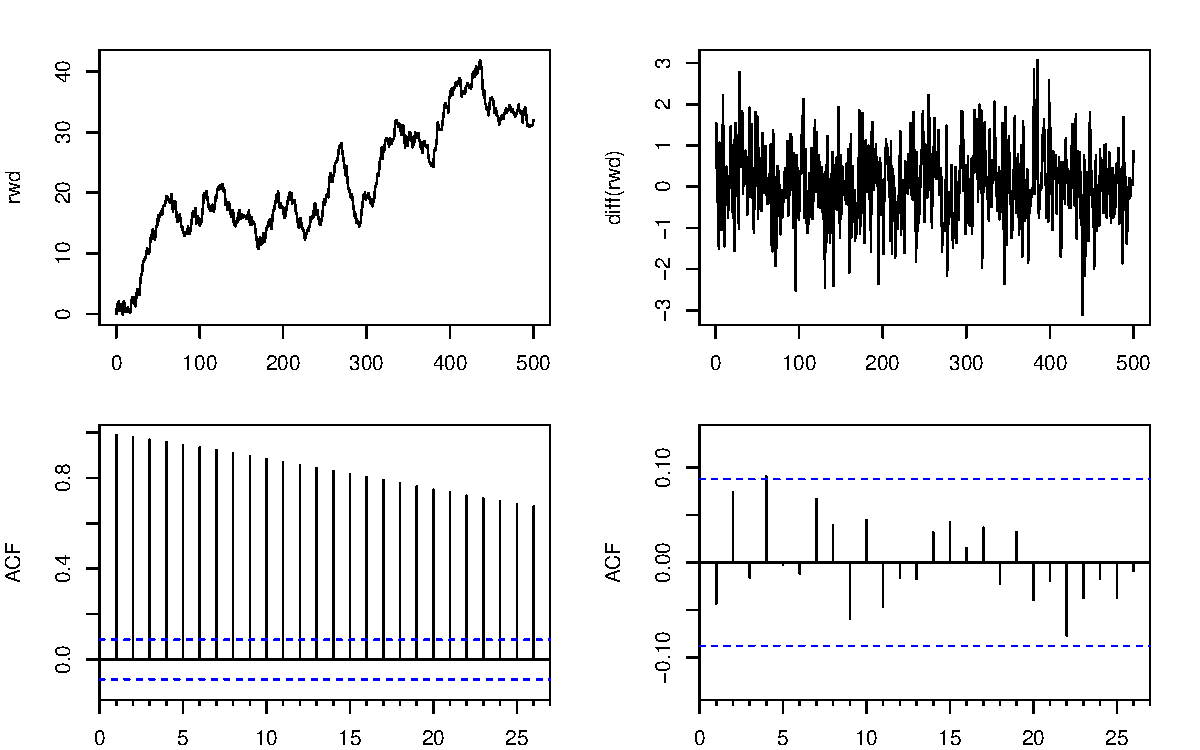
\includegraphics{Lec9_files/figure-beamer/unnamed-chunk-2-1.pdf}

\end{frame}

\begin{frame}{Over differencing}

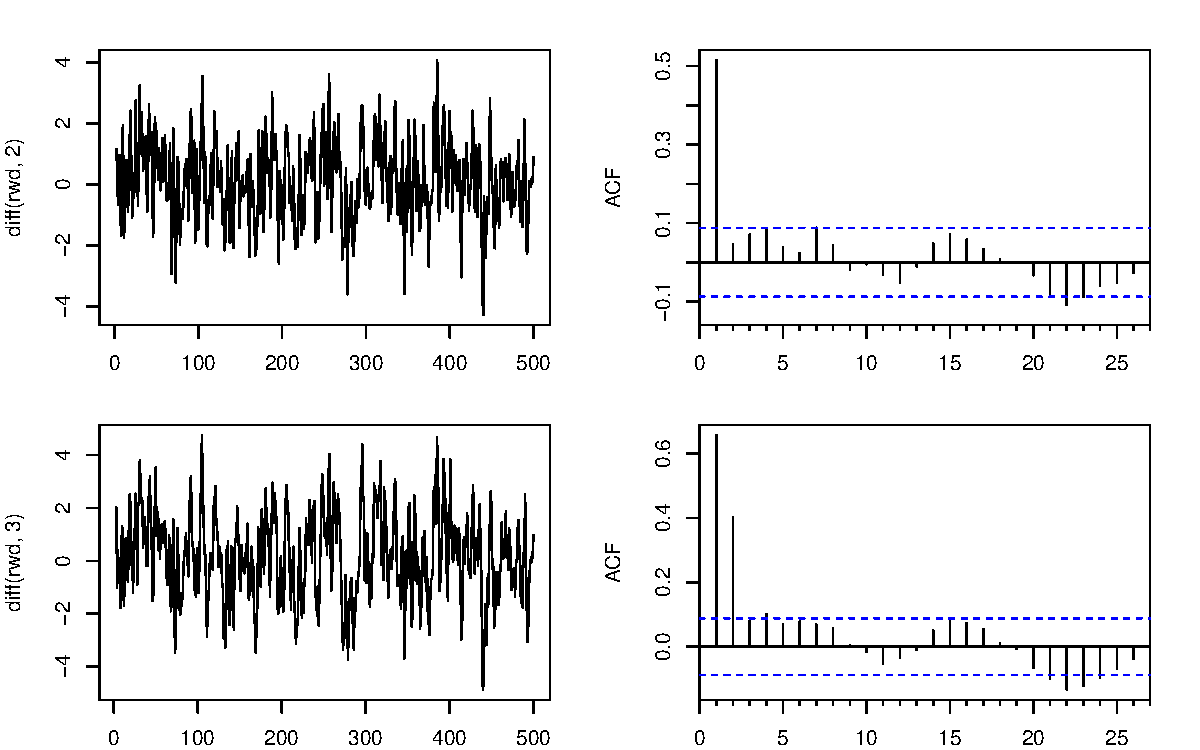
\includegraphics{Lec9_files/figure-beamer/unnamed-chunk-3-1.pdf}

\end{frame}

\begin{frame}{AR or MA?}

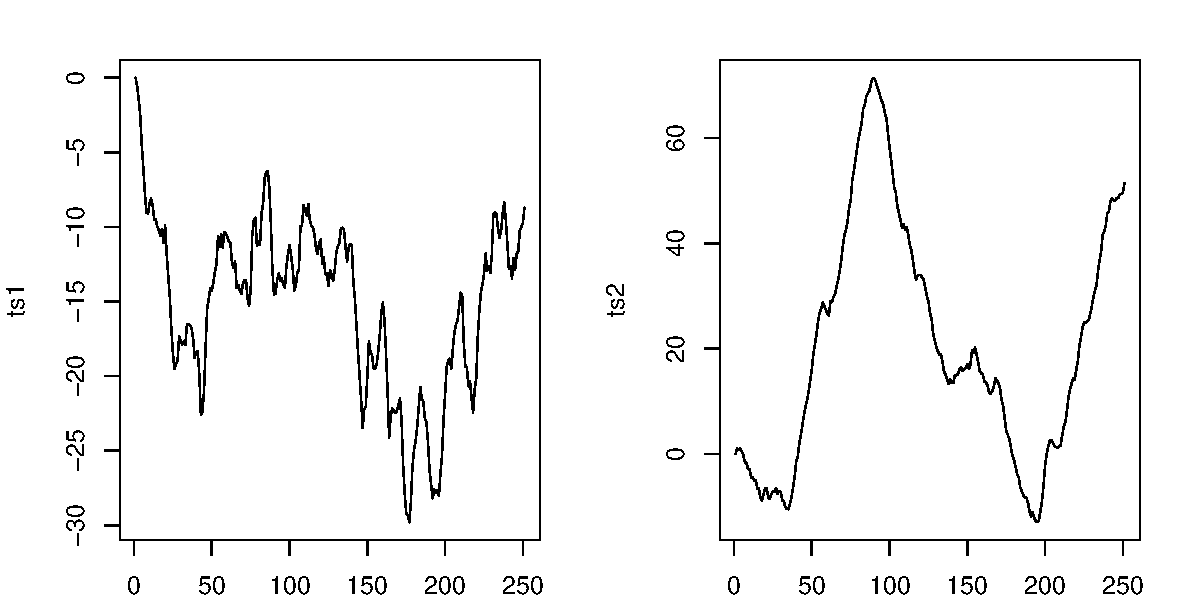
\includegraphics{Lec9_files/figure-beamer/unnamed-chunk-4-1.pdf}

\end{frame}

\begin{frame}{EDA}

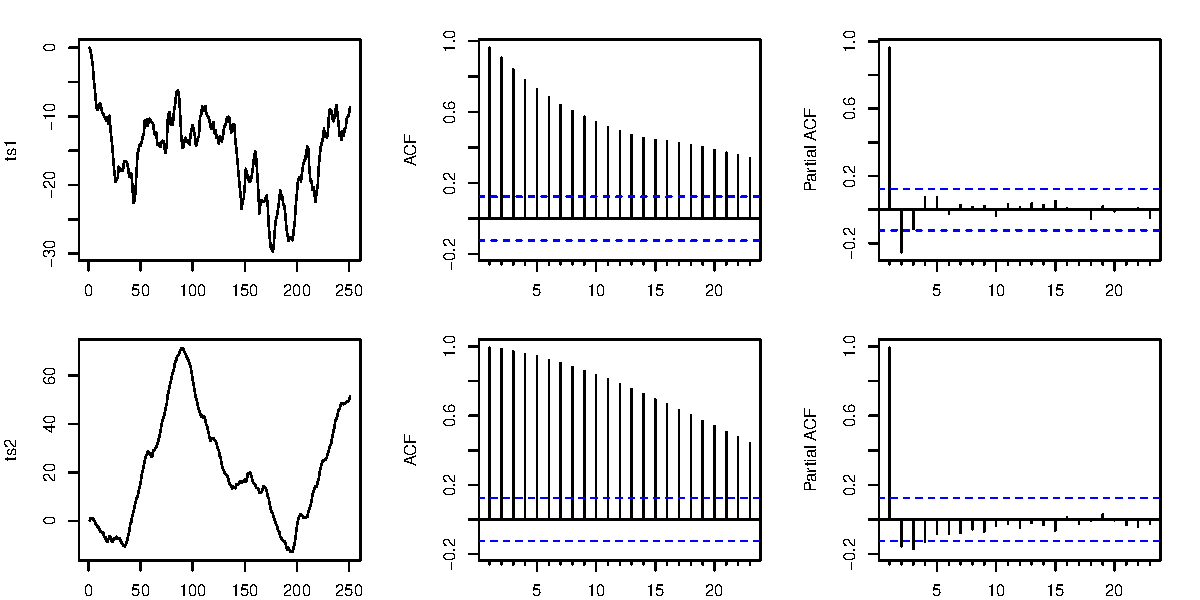
\includegraphics{Lec9_files/figure-beamer/unnamed-chunk-5-1.pdf}

\end{frame}

\begin{frame}{\texttt{ts1} - Finding \(d\)}

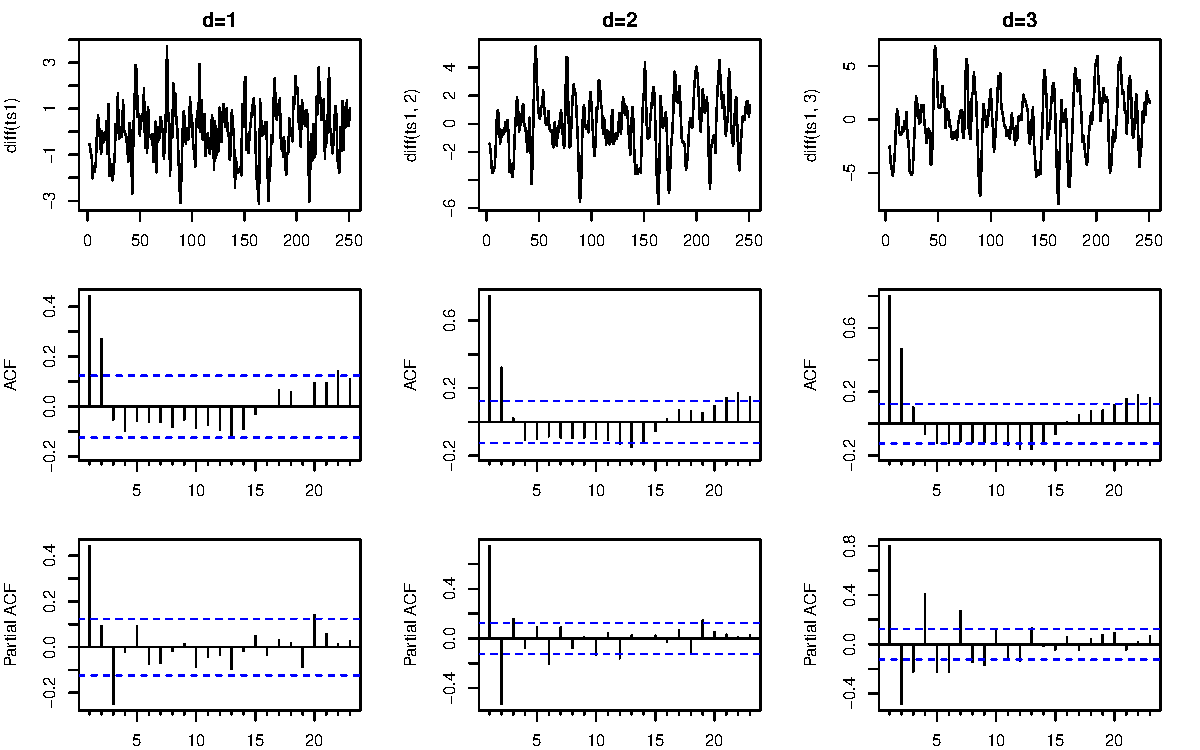
\includegraphics{Lec9_files/figure-beamer/unnamed-chunk-6-1.pdf}

\end{frame}

\begin{frame}{\texttt{ts2} - Finding \(d\)}

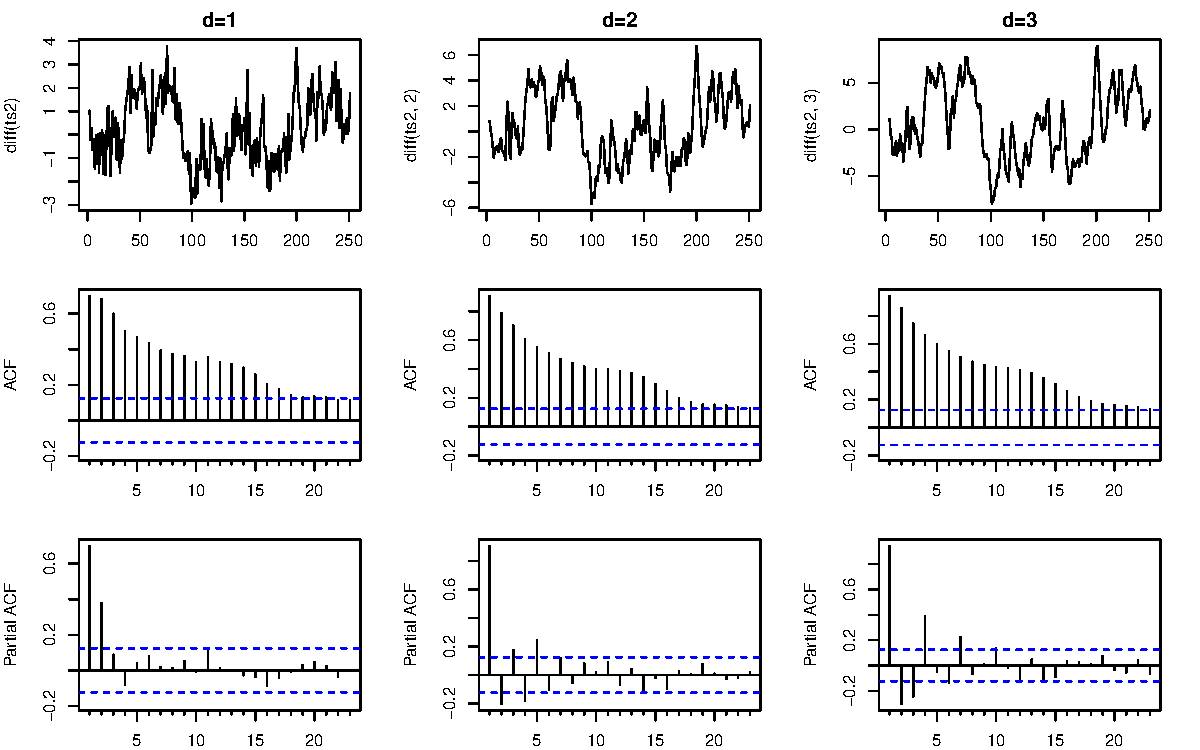
\includegraphics{Lec9_files/figure-beamer/unnamed-chunk-7-1.pdf}

\end{frame}

\begin{frame}{\texttt{ts1} - Models}

\begin{longtable}[]{@{}rrrrr@{}}
\toprule
p & d & q & AIC & BIC\tabularnewline
\midrule
\endhead
0 & 1 & 2 & 729.43 & 740.00\tabularnewline
1 & 1 & 2 & 731.23 & 745.31\tabularnewline
2 & 1 & 2 & 731.57 & 749.18\tabularnewline
2 & 1 & 1 & 744.29 & 758.38\tabularnewline
2 & 1 & 0 & 747.55 & 758.12\tabularnewline
1 & 1 & 0 & 747.61 & 754.65\tabularnewline
1 & 1 & 1 & 748.65 & 759.21\tabularnewline
0 & 1 & 1 & 764.98 & 772.02\tabularnewline
0 & 1 & 0 & 800.43 & 803.95\tabularnewline
\bottomrule
\end{longtable}

\end{frame}

\begin{frame}{\texttt{ts2} - Models}

\begin{longtable}[]{@{}rrrrr@{}}
\toprule
p & d & q & AIC & BIC\tabularnewline
\midrule
\endhead
2 & 1 & 0 & 683.12 & 693.68\tabularnewline
1 & 1 & 2 & 683.25 & 697.34\tabularnewline
2 & 1 & 1 & 683.83 & 697.92\tabularnewline
2 & 1 & 2 & 685.06 & 702.67\tabularnewline
1 & 1 & 1 & 686.38 & 696.95\tabularnewline
1 & 1 & 0 & 719.16 & 726.20\tabularnewline
0 & 1 & 2 & 754.66 & 765.22\tabularnewline
0 & 1 & 1 & 804.44 & 811.48\tabularnewline
0 & 1 & 0 & 890.32 & 893.85\tabularnewline
\bottomrule
\end{longtable}

\end{frame}

\begin{frame}[fragile,t]{\texttt{ts1} - Model Choice}

\begin{Shaded}
\begin{Highlighting}[]
\KeywordTok{Arima}\NormalTok{(ts1, }\DataTypeTok{order =} \KeywordTok{c}\NormalTok{(}\DecValTok{0}\NormalTok{,}\DecValTok{1}\NormalTok{,}\DecValTok{2}\NormalTok{))}
\NormalTok{## Series: ts1 }
\NormalTok{## ARIMA(0,1,2)                    }
\NormalTok{## }
\NormalTok{## Coefficients:}
\NormalTok{##          ma1     ma2}
\NormalTok{##       0.4138  0.4319}
\NormalTok{## s.e.  0.0547  0.0622}
\NormalTok{## }
\NormalTok{## sigma^2 estimated as 1.064:  log likelihood=-361.72}
\NormalTok{## AIC=729.43   AICc=729.53   BIC=740}
\end{Highlighting}
\end{Shaded}

\end{frame}

\begin{frame}[fragile,t]{\texttt{ts2} - Model Choice}

\begin{Shaded}
\begin{Highlighting}[]
\KeywordTok{Arima}\NormalTok{(ts2, }\DataTypeTok{order =} \KeywordTok{c}\NormalTok{(}\DecValTok{2}\NormalTok{,}\DecValTok{1}\NormalTok{,}\DecValTok{0}\NormalTok{))}
\NormalTok{## Series: ts2 }
\NormalTok{## ARIMA(2,1,0)                    }
\NormalTok{## }
\NormalTok{## Coefficients:}
\NormalTok{##          ar1     ar2}
\NormalTok{##       0.4392  0.3770}
\NormalTok{## s.e.  0.0587  0.0587}
\NormalTok{## }
\NormalTok{## sigma^2 estimated as 0.8822:  log likelihood=-338.56}
\NormalTok{## AIC=683.12   AICc=683.22   BIC=693.68}
\end{Highlighting}
\end{Shaded}

\end{frame}

\begin{frame}{Residuals}

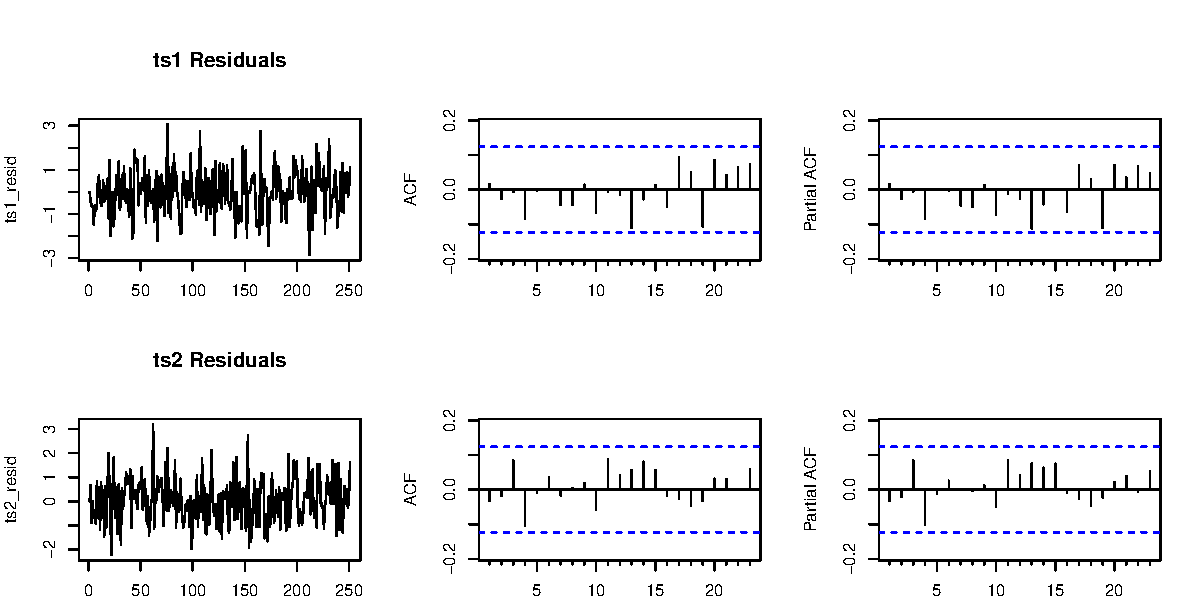
\includegraphics{Lec9_files/figure-beamer/unnamed-chunk-12-1.pdf}

\end{frame}

\section{Electrical Equipment Sales}\label{electrical-equipment-sales}

\begin{frame}{Data}

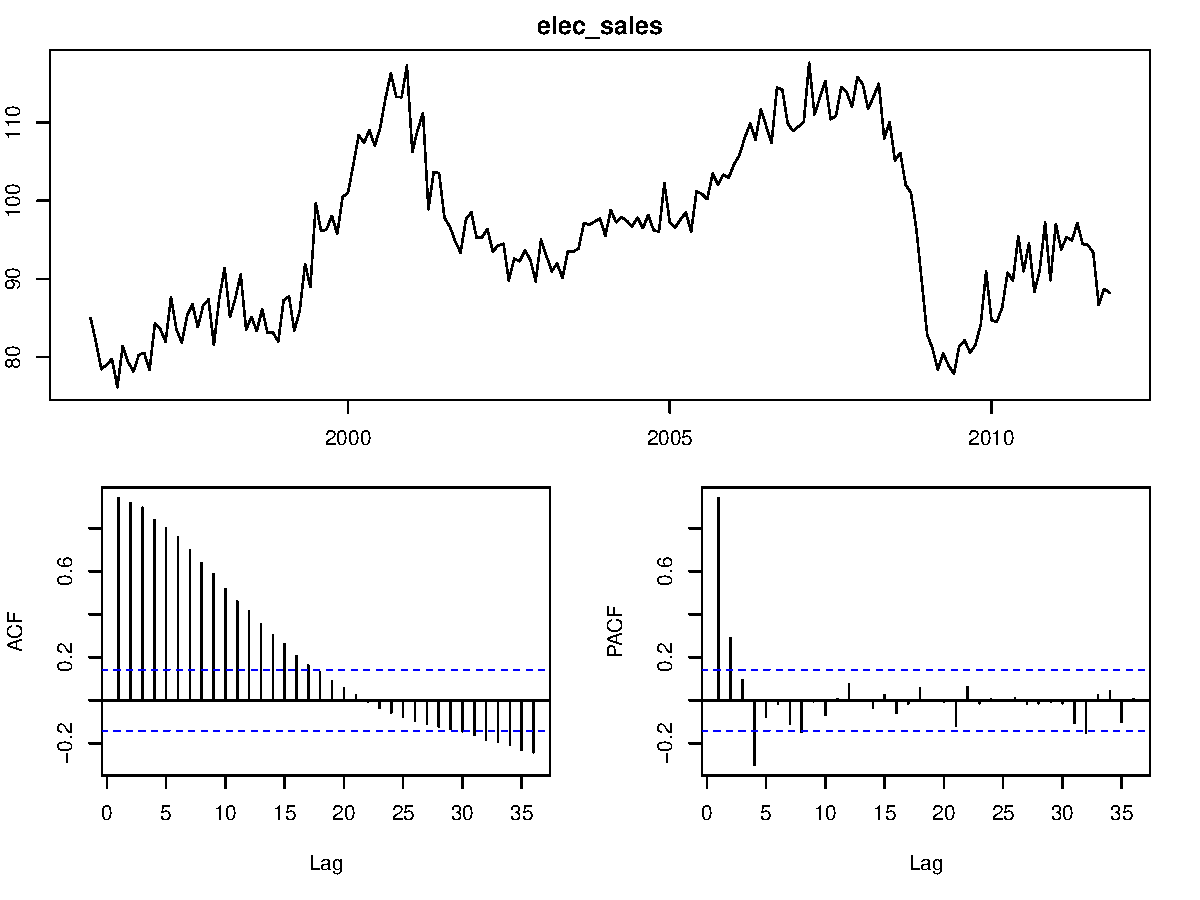
\includegraphics{Lec9_files/figure-beamer/unnamed-chunk-13-1.pdf}

\end{frame}

\begin{frame}{1st order differencing}

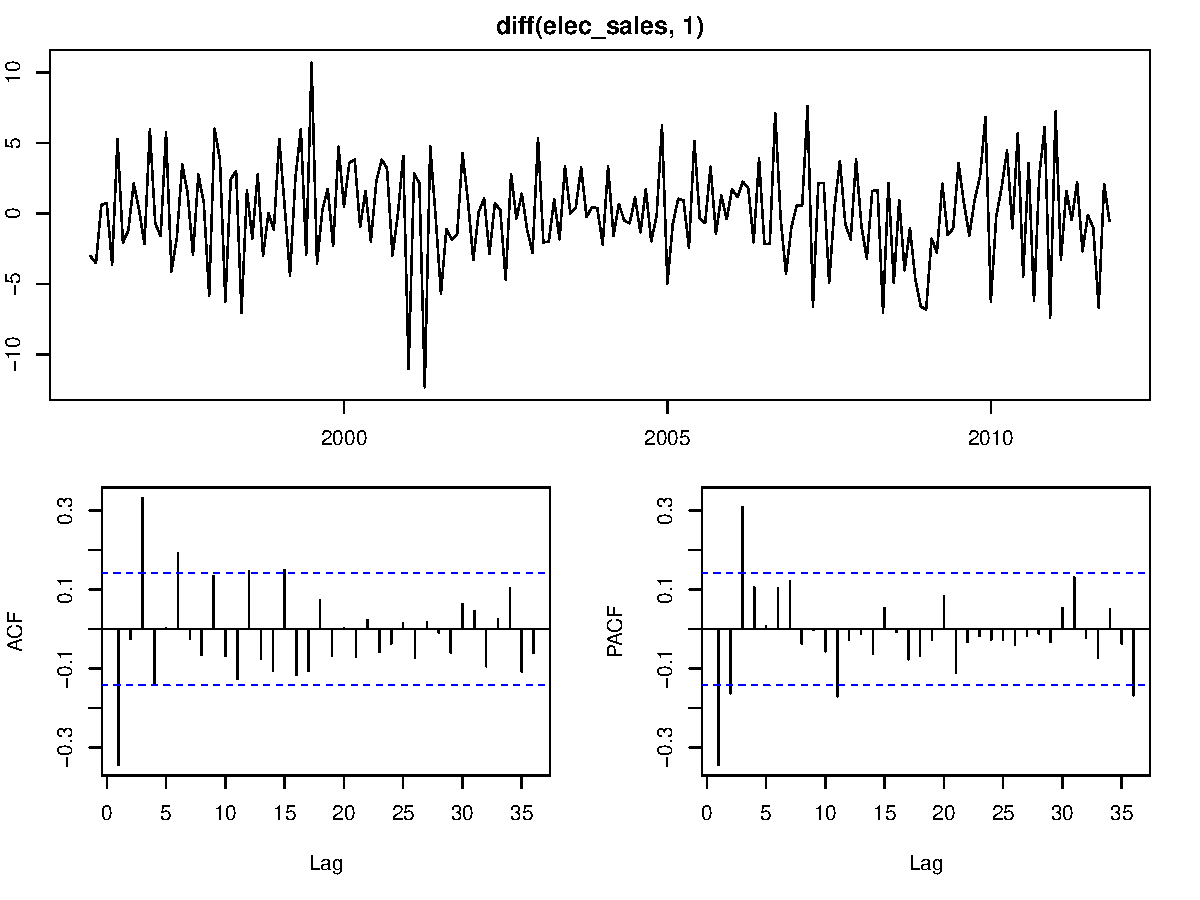
\includegraphics{Lec9_files/figure-beamer/unnamed-chunk-14-1.pdf}

\end{frame}

\begin{frame}{2nd order differencing}

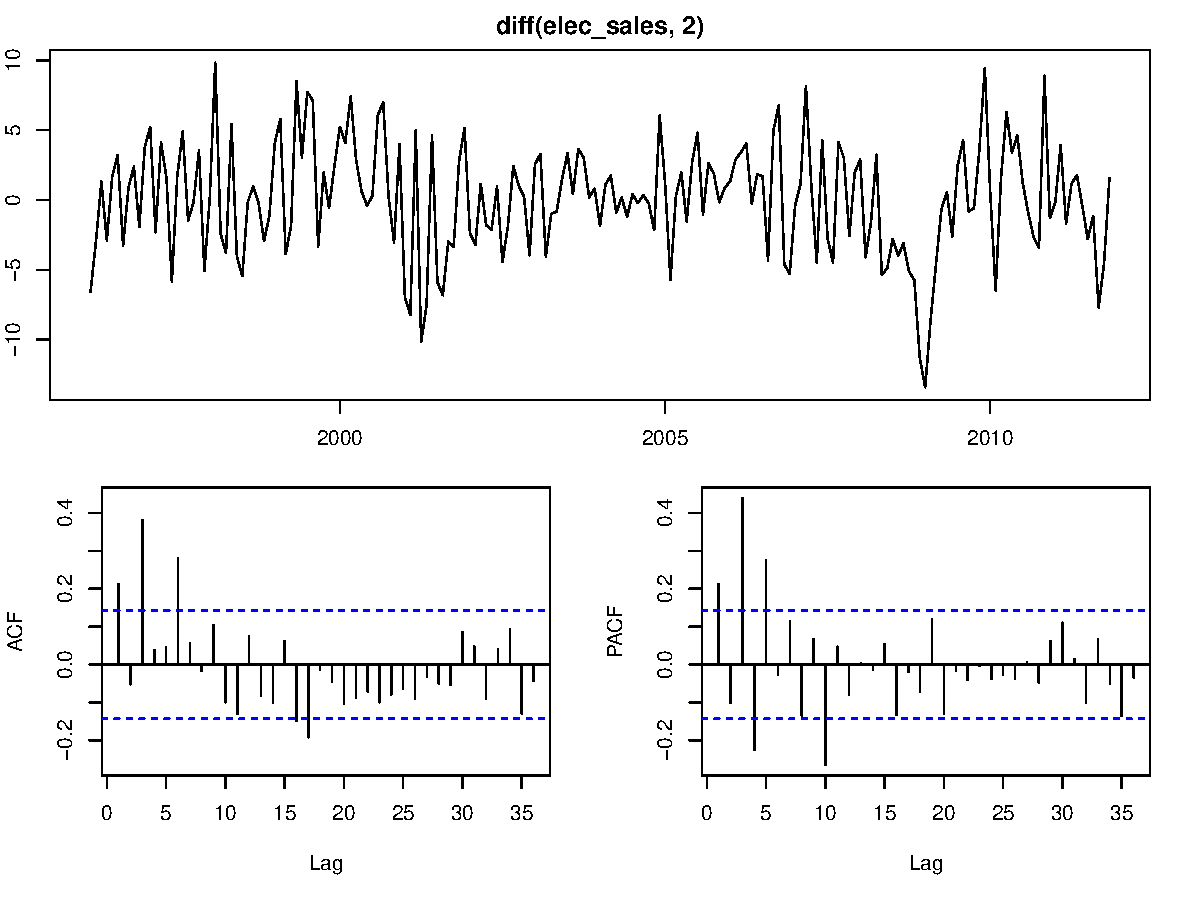
\includegraphics{Lec9_files/figure-beamer/unnamed-chunk-15-1.pdf}

\end{frame}

\begin{frame}[fragile,t]{Model}

\begin{Shaded}
\begin{Highlighting}[]
\KeywordTok{Arima}\NormalTok{(elec_sales, }\DataTypeTok{order =} \KeywordTok{c}\NormalTok{(}\DecValTok{3}\NormalTok{,}\DecValTok{1}\NormalTok{,}\DecValTok{0}\NormalTok{))}
\NormalTok{## Series: elec_sales }
\NormalTok{## ARIMA(3,1,0)                    }
\NormalTok{## }
\NormalTok{## Coefficients:}
\NormalTok{##           ar1      ar2     ar3}
\NormalTok{##       -0.3488  -0.0386  0.3139}
\NormalTok{## s.e.   0.0690   0.0736  0.0694}
\NormalTok{## }
\NormalTok{## sigma^2 estimated as 9.853:  log likelihood=-485.67}
\NormalTok{## AIC=979.33   AICc=979.55   BIC=992.32}
\end{Highlighting}
\end{Shaded}

\end{frame}

\begin{frame}[fragile]{Residuals}

\begin{Shaded}
\begin{Highlighting}[]
\KeywordTok{Arima}\NormalTok{(elec_sales, }\DataTypeTok{order =} \KeywordTok{c}\NormalTok{(}\DecValTok{3}\NormalTok{,}\DecValTok{1}\NormalTok{,}\DecValTok{0}\NormalTok{)) }\OperatorTok\StringTok{ }\KeywordTok{residuals}\NormalTok{() }\OperatorTok\StringTok{ }\KeywordTok{tsdisplay}\NormalTok{(}\DataTypeTok{points=}\OtherTok{FALSE}\NormalTok{)}
\end{Highlighting}
\end{Shaded}

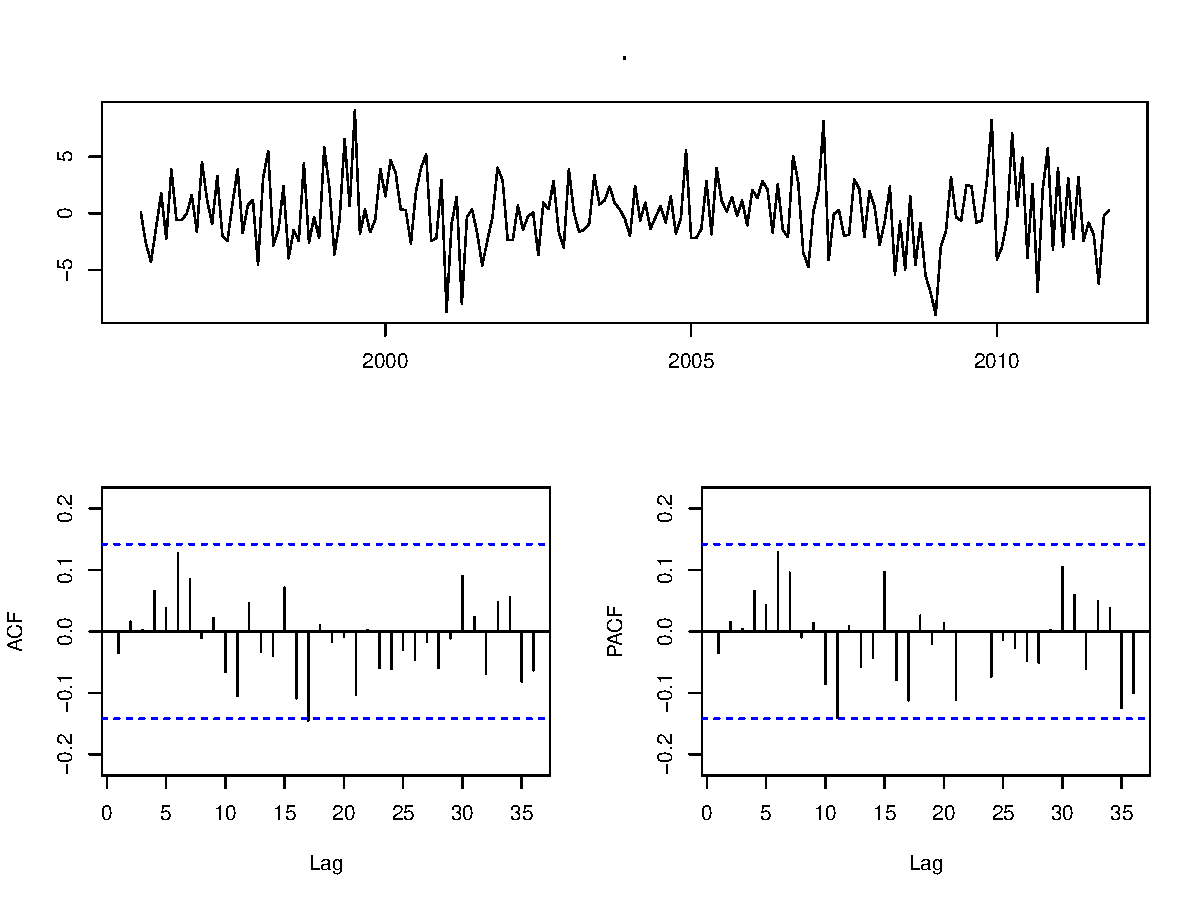
\includegraphics{Lec9_files/figure-beamer/unnamed-chunk-18-1.pdf}

\end{frame}

\begin{frame}[fragile]{Model Comparison}

\begin{Shaded}
\begin{Highlighting}[]
\KeywordTok{Arima}\NormalTok{(elec_sales, }\DataTypeTok{order =} \KeywordTok{c}\NormalTok{(}\DecValTok{3}\NormalTok{,}\DecValTok{1}\NormalTok{,}\DecValTok{0}\NormalTok{))}\OperatorTok{$}\NormalTok{aic}
\NormalTok{## [1] 979.3314}

\KeywordTok{Arima}\NormalTok{(elec_sales, }\DataTypeTok{order =} \KeywordTok{c}\NormalTok{(}\DecValTok{3}\NormalTok{,}\DecValTok{1}\NormalTok{,}\DecValTok{1}\NormalTok{))}\OperatorTok{$}\NormalTok{aic}
\NormalTok{## [1] 978.1664}

\KeywordTok{Arima}\NormalTok{(elec_sales, }\DataTypeTok{order =} \KeywordTok{c}\NormalTok{(}\DecValTok{4}\NormalTok{,}\DecValTok{1}\NormalTok{,}\DecValTok{0}\NormalTok{))}\OperatorTok{$}\NormalTok{aic}
\NormalTok{## [1] 978.9048}

\KeywordTok{Arima}\NormalTok{(elec_sales, }\DataTypeTok{order =} \KeywordTok{c}\NormalTok{(}\DecValTok{2}\NormalTok{,}\DecValTok{1}\NormalTok{,}\DecValTok{0}\NormalTok{))}\OperatorTok{$}\NormalTok{aic}
\NormalTok{## [1] 996.6795}
\end{Highlighting}
\end{Shaded}

\end{frame}

\begin{frame}[fragile]{Model fit}

\begin{Shaded}
\begin{Highlighting}[]
\KeywordTok{plot}\NormalTok{(elec_sales, }\DataTypeTok{lwd=}\DecValTok{2}\NormalTok{, }\DataTypeTok{col=}\KeywordTok{adjustcolor}\NormalTok{(}\StringTok{"blue"}\NormalTok{, }\DataTypeTok{alpha.f=}\FloatTok{0.75}\NormalTok{))}
\KeywordTok{Arima}\NormalTok{(elec_sales, }\DataTypeTok{order =} \KeywordTok{c}\NormalTok{(}\DecValTok{3}\NormalTok{,}\DecValTok{1}\NormalTok{,}\DecValTok{0}\NormalTok{)) }\OperatorTok\StringTok{ }\KeywordTok{fitted}\NormalTok{() }\OperatorTok\StringTok{ }\KeywordTok{lines}\NormalTok{(}\DataTypeTok{col=}\KeywordTok{adjustcolor}\NormalTok{(}\StringTok{'red'}\NormalTok{,}\DataTypeTok{alpha.f=}\FloatTok{0.75}\NormalTok{),}\DataTypeTok{lwd=}\DecValTok{2}\NormalTok{)}
\end{Highlighting}
\end{Shaded}

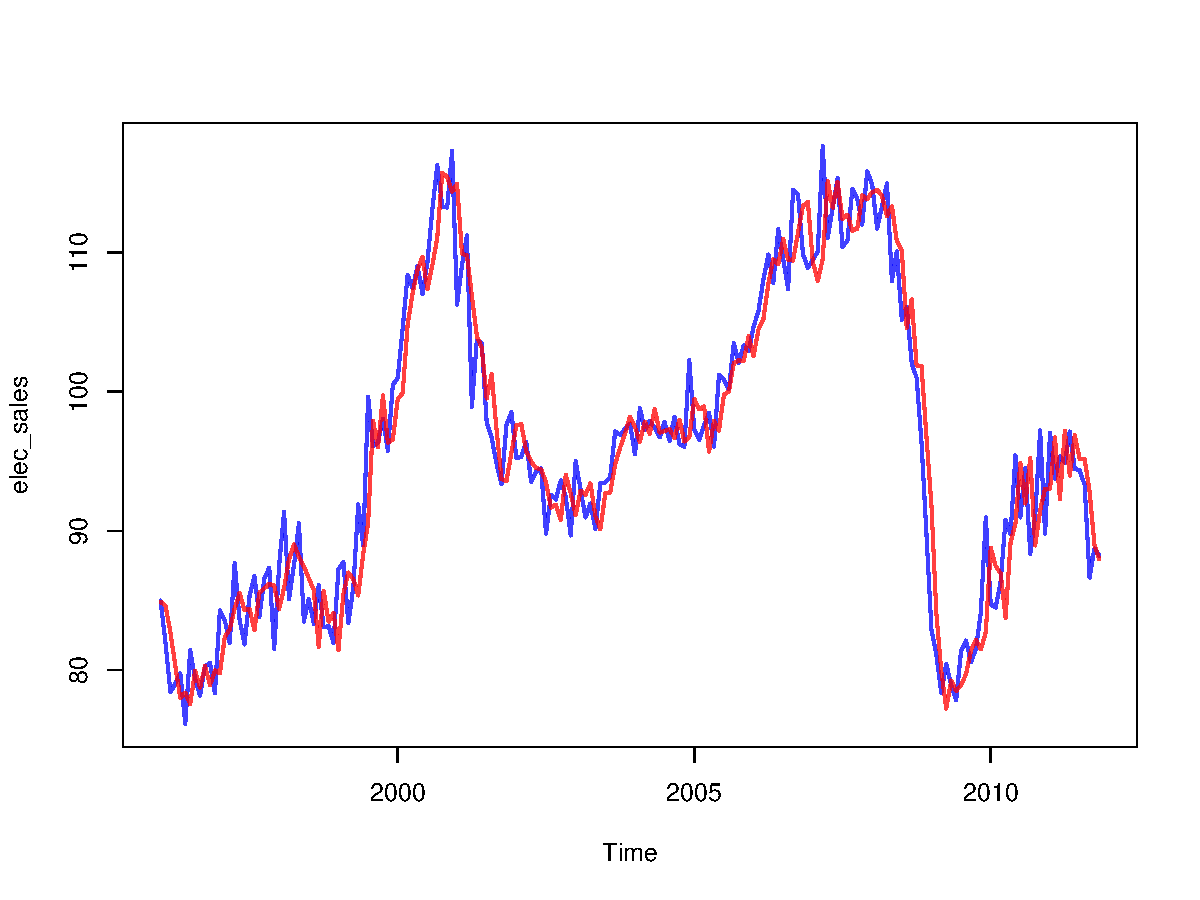
\includegraphics{Lec9_files/figure-beamer/unnamed-chunk-20-1.pdf}

\end{frame}

\begin{frame}[fragile]{Model forecast}

\begin{Shaded}
\begin{Highlighting}[]
\KeywordTok{Arima}\NormalTok{(elec_sales, }\DataTypeTok{order =} \KeywordTok{c}\NormalTok{(}\DecValTok{3}\NormalTok{,}\DecValTok{1}\NormalTok{,}\DecValTok{0}\NormalTok{)) }\OperatorTok\StringTok{ }\KeywordTok{forecast}\NormalTok{() }\OperatorTok\StringTok{ }\KeywordTok{plot}\NormalTok{()}
\end{Highlighting}
\end{Shaded}

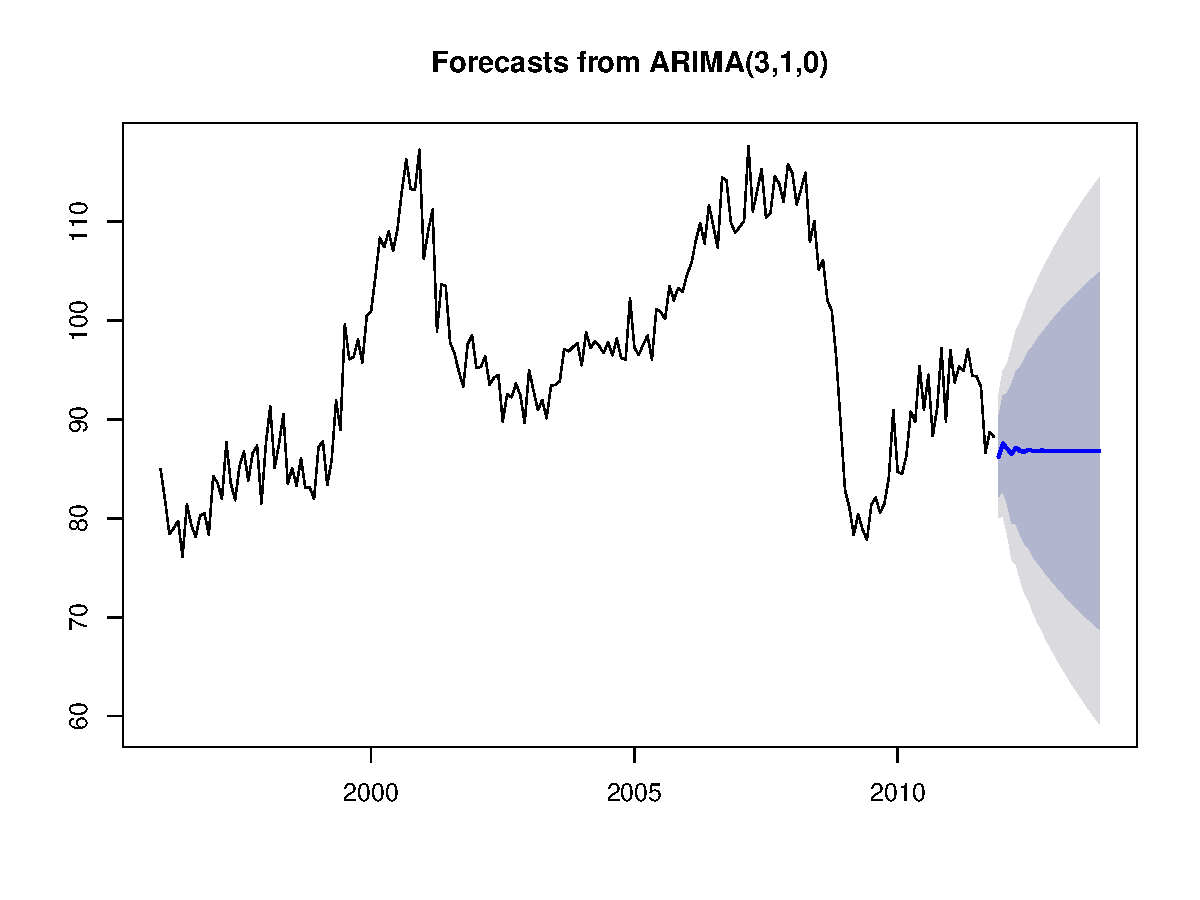
\includegraphics{Lec9_files/figure-beamer/unnamed-chunk-21-1.pdf}

\end{frame}

\begin{frame}[t]{General Guidance}

\begin{enumerate}
\def\labelenumi{\arabic{enumi}.}
\item
  Positive autocorrelations out to a large number of lags usually
  indicates a need for differencing
\item
  Slightly too much or slightly too little differencing can be corrected
  by adding AR or MA terms respectively.
\item
  A model with no differencing usually includes a constant term, a model
  with two or more orders (rare) differencing usually does not include a
  constant term.
\item
  After differencing, if the PACF has a sharp cutoff then consider
  adding AR terms to the model.
\item
  After differencing, if the ACF has a sharp cutoff then consider adding
  an MA term to the model.
\item
  It is possible for an AR term and an MA term to cancel each other's
  effects, so try models with one fewer AR term and one fewer MA term.
\end{enumerate}

\scriptsize{Based on rules from \url{https://people.duke.edu/~rnau/411arim2.htm} and \url{https://people.duke.edu/~rnau/411arim3.htm}}

\end{frame}

\end{document}
